\documentclass{sigchi}

% If not to appear in proceedings, remove ``Permission'' sentence or comment out these two lines for final version and replace by ``Copyright is held by the author(s)
\toappear{\small 
%Permission to make digital or hard copies of all or part of this work for personal or classroom use is granted without fee provided that copies are not made or distributed for profit or commercial advantage and that copies bear this notice and the full citation on the first page. To copy otherwise, or republish, to post on servers or to redistribute to lists, requires prior specific permission and/or a fee. \newline   \emph{WebSci'13}, May 1 -- May 5, 2013, Paris, France.\\ ACM 978-1-4503-1889-1.
}
\pagenumbering{arabic}% Arabic page numbers for submission. 

% Use \toappear{...} to override the default ACM copyright statement (e.g. for preprints).

% Load basic packages
\usepackage{balance}  % to better equalize the last page
\usepackage{graphics} % for EPS, load graphicx instead
\usepackage{times}    % comment if you want LaTeX's default font
\usepackage{url}      % llt: nicely formatted URLs

% llt: Define a global style for URLs, rather that the default one
\makeatletter
\def\url@leostyle{%
  \@ifundefined{selectfont}{\def\UrlFont{\sf}}{\def\UrlFont{\small\bf\ttfamily}}}
\makeatother
\urlstyle{leo}


% To make various LaTeX processors do the right thing with page size.
\def\pprw{8.5in}
\def\pprh{11in}
\special{papersize=\pprw,\pprh}
\setlength{\paperwidth}{\pprw}
\setlength{\paperheight}{\pprh}
\setlength{\pdfpagewidth}{\pprw}
\setlength{\pdfpageheight}{\pprh}

% Make sure hyperref comes last of your loaded packages, 
% to give it a fighting chance of not being over-written, 
% since its job is to redefine many LaTeX commands.
\usepackage[pdftex]{hyperref}
\hypersetup{
pdftitle={SIGCHI Conference Proceedings Format},
pdfauthor={LaTeX},
pdfkeywords={SIGCHI, proceedings, archival format},
bookmarksnumbered,
pdfstartview={FitH},
colorlinks,
citecolor=black,
filecolor=black,
linkcolor=black,
urlcolor=black,
breaklinks=true,
}

% create a shortcut to typeset table headings
\newcommand\tabhead[1]{\small\textbf{#1}}


% End of preamble. Here it comes the document.
\begin{document}

\title{Hacking the Dynamics of Data Science \\ \vspace{0.3cm} {\LARGE {\bf Watching under the hood of open and reproducible science}} \\ \vspace{0.8cm} {\large \bf -- Preliminary version. Please do not share without authors consent. --} \vspace{0.5cm}}

% Note that submissions are blind, so author information should be omitted
\numberofauthors{2}
\author{
% 1st Author
\alignauthor 
Thomas Maillart\\
    \affaddr{School of Information}\\
    \affaddr{UC Berkeley}\\
    \affaddr{102 South Hall, Berkeley, CA 94720}\\
    \email{maillart@ischool.berkeley.edu}
% 2nd Author
\alignauthor 
Charlotte Cabasse-Mazel\\
    \affaddr{Berkeley Institute for Data Science}\\
    \affaddr{UC Berkeley}\\
    \affaddr{190 Doe Library, Berkeley, CA 94720}\\
    \email{charlottecabasse@berkeley.edu}
}
%    \affaddr{Optional phone number}    
%  \alignauthor 3rd Author Name\\
%    \affaddr{Affiliation}\\
%    \affaddr{Address}\\
%    \email{e-mail address}\\
%    \affaddr{Optional phone number}
% Teaser figure can go here
%\teaser{
%  \centering
%  \includegraphics{Figure1}
%  \caption{Teaser Image}
%  \label{fig:teaser}
%}

\maketitle

\begin{abstract}
As academic research gets increasingly computational, distributed, interdisciplinary and open, studying the practice of science requires to account for heterogeneous and self-organized online communities, which leave complex -- yet data-rich -- footprints. Considering a community of scientists committed in open and reproducible science, and active across domains of cosmology, astronomy and astrophysics, we studied the dynamics triggered by a specific community gathering: the Astro Hack Week 2014. We found that past the initial impulse, the Astro Hack Week community triggered long-term follow-up scientific activity, stemming from a socio-technical assemblage of exposure to a new set of collective scientific practices, such as hackathons, growing adoption of collaborative tools and methods across disciplines (e.g., machine learning, statistics, computing). Our approach, combining modeling of social dynamics and ethnography, helps inform how communities build-up and gather around common goals, as well as practices, for a more open and reproducible science.

\end{abstract}

%\keywords{
%	Guides; instructions; author's kit; conference publications;
%	keywords should be separated by a semi-colon.
%	\\\textcolor{red}{Mandatory section to be included in your final version.}
%}

\category{H.5.3}{[Information Systems]: Group and Organization Interfaces}{computer-supported collaborative work}

%\terms{
%	Human Factors; Design; Measurement. 
%	If you choose more than one ACM General Term, 
%	separate the terms with a semi-colon.
%\\
%\textcolor{red}{If you choose more than one ACM General Term, 
%separate the terms with a semi-colon. See list of ACM terms at:
%\url{http://www.sheridanprinting.com/sigchi/generalterms.htm}.
%Optional section to be included in your final version.}
%}

\section{Introduction}
In recent years, forms of collaborations and cooperation in science have been transformed. As computing tools get generalized in larger scientific communities, the lab, which used to be studied in the classic Science Technology and Society (STS) literature \cite{latour1987science,houdart2008cour}, has been progressively replaced by new settings, redefining the standards \cite{galison1996disunity,kitchin2014big} on the way science is, and how it should be practiced \cite{calvert2013collaboration,leonelli2012introduction}. Additionally, while the last decades have been dominated by closed-source scientific software (e.g., MatLab, Mathematica), number of tools and libraries for research nowadays build upon community maintained open source programs and libraries, such as R, Numpy, Scipy, IPython Notebook, or Jupyter. These libraries are also increasingly publicly shared, for peer-review, for thorough reproduction of research results, and for reuse in other contexts and by other researchers. The lines between scientific software and libraries used for research are increasingly blurred, into the same complex ecosystem of code sharing. As a consequence of these emergent scientific practices, scientific tools are also increasingly achieved through the integration of heterogeneous perspectives and computational methods. In this context, the role of a researcher gets multiplied and diversified as he becomes a collaborator of his domain sciences, but also a contributor, a debugger, a user, and a promoter of a scientific library maintained by an open software community, in addition to more traditional tasks, such as conceiving research protocols, gathering data, testing hypotheses, and presenting results in scientific articles.

While open collaboration, as well as open and reproducible science, seems to be a genuine means and feature witnessed broadly in highly connected societies \cite{benkler2011penguin}, for the quantitative researcher, understanding the complex dynamics shaping self-organized communities has remained a challenge, despite the abundance of publicly available data available. Most often, large scale data mining quantitative studies lack sufficient context to extract the meaning of actions performed, while qualitative studies, focused on extracting context, might seem too partial and focused, thus preventing from getting a better big picture without losing context. 

However, the growing use of collaborative tools for scientific research has generated large amounts of data, which challenge the enduring lack of communication between qualitative and quantitative research methods.  As Venturini et al. recalled \cite{venturini2015fill}, traceability and contextualization of the data allow the emergence of a new form of quantitatively informed ethnography, particularly relevant to study the complex dynamics of scientific collaboration that social coding platforms, such as GitHub. Here, we address this methodological gap, by combining state-of-the-art modeling of social dynamics, with ethnography to analyze how a small group of scientists promote more open and reproducible science practices, in order to build epistemic communities and collaborative platforms in academia \cite{calvert2013collaboration}.

In this paper, we focus on a specific event, the Astro Hack Week, which was held at the University of Washington, from September 15-19, 2014. A large quantity of events that punctuated the Astro Hack Week, have been recorded on GitHub \cite{github}, a social coding platform, which rapidly transforms the way in which scientists are collaborating \cite{gerson2013integration}. Social coding platforms are promoting new ways to work together in data driven environments, where science is being redefined with some value of openness and reproducibility \cite{ducheneaut2005socialization}, including code accessibility and verification \cite{hayden2015rule,proebsting2015repeatability}. Looking at the dynamics of GitHub contributions by Astro Hack Week actors, and framing them in the socio-technical context in which they have emerged, we show that past the initial impulse, the Astro Hack Week triggered mid- term and long-term follow-up activity. We illustrate how this activity is only qualitatively tangentially related to the Astro Hack Week, and rather stems from the exposure to a new practice of science, and from the build-up of new social ties.

The rest of this paper is organized as follows. We first further expose the reader to the literature in relation with the emergence of platforms and tools, tuned for a rather self-organized practice of science, coming from the complex dynamics of computer supported collaborative work (CSCW) and Science and Technologies Studies (STS). We then present a method, which combines qualitative and quantitative analysis and in-depth modeling of actions taken by participants, before, during and after the Astro Hack Week. Data employed and results are then presented, and discussed. We finally conclude with limitations and future research directions.

%The way open and reproducible science evolves is a challenge, if not a paradigm change, for STS studies. In recent years, however, the development of collaborative tools for scientific research has generated a large amount of data that may help bridging the gap between qualitative and quantitative methods. As Tommaso et al. \cite{tommaso2015} {\bf [missing reference for Tommaso]} recalled, both the phenomenon of traceability and the capacity to re contextualized the data that have been collected allow the emergence of a new form of ethnography, which is both qualitatively and quantitatively informed. Such method seems particularly relevant to study the complex dynamics of scientific collaboration that social coding platforms, such as GitHub, are making possible and visible in the context of computational intensive scientific projects. 


%Like for most instances of open collaboration, academia needs to build a strong and large community of scientists. Important efforts have been undertaken across fields by universities (e.g., Software Carpentry \cite{software_carpentry}, or by discipline (across institutions) \cite{calvert2013collaboration}. In this paper, we focus on the Astro Hack Week (AstroWeek), which was held at the University of Washington, from September 15-19, 2014, with the support the Moore Foundation, the Sloan Foundation, and the UW eScience Institute. A large quantity of events that punctuated the AstroWeek, have been recorded on GitHub \cite{github}, a social coding platform, which rapidly transforms the way in which scientists are collaborating \cite{gerson2013integration}. GitHub is promoting new way to collaborate in data driven scientific environment where science is being redefined with some value of openness and reproducibility \cite{ducheneaut2005socialization} -- which include code accessibility  and verification \cite{hayden2015rule,proebsting2015repeatability}.

%Looking at the dynamics of contributions by actors, we show that past the initial impulse, AstroWeek triggered long-term follow-up activity. We illustrate how this long-term activity is only qualitatively tangentially related to the AstroWeek, and rather stems from the exposure to a new practice of science, and from the build-up of new social ties. We also document the ``costs"  of senior data scientists spending time teaching data science to lay participants.



%During the days the time was divided between the sessions dedicated of teaching and learning of coding, statistics, and skills required for data analysis of large data set and the afternoon where dedicated to specific projects and breakout sessions. 


%To address the problem of community building and onboarding, we study the community of astronomers {\bf [astrophysicists? cosmologists?]}, learning and practicing data science. In particular, we focus on the Astro Hack Week, which was held at the University of Washington on September 15-19, 2014 (with the support the Moore Foundation, the Sloan Foundation, and the UW eScience Institute). 


%Here, we shall document how a one-week hackathon (the Astro Hack Week), organized for the purpose of engaging scientists in the practice of open and reproducible data science, has short-, mid-term and long-term spillovers {\bf [not sure for the long-term]}, as a result of critical cascades of repository creations and forks \cite{}, as well as contributions to broader data science community {\bf [it's not clear here, but the goal is to convey the idea that while projects during the Astro Hack Week, may be short lived, the mere fact of having people interact (physically), creates opportunities for future stand-alone contributions or even collaborations (c.f., testimony of Kyle)]}


\section{Background}
As computing tools get generalized in larger scientific communities, the lab has progressively evolved with new tools, but also with a refashioned vision. The move towards more open and reproducible practice of science, supported by online collaboration tools, is one of the many artifacts of the fast-paced evolution of science practice. It should not be a surprise that scientific practice has finally reconnected with the open collaboration approach -- the generalized version of open source software development, which was itself deeply inspired by the scientific approach \cite{raymond1999cathedral}. 

Challenges faced by open and reproducible science are, in many ways, similar to those faced by computer supported collaborative work (CSCW). These research and practice challenges include, understanding motives deeply governed by intrinsic motivation \cite{vonKrogh2012}, solving social dilemma in complex settings \cite{baldwin2007}, and overcoming technical and social barriers, which may prevent the growth and the renewal of communities \cite{halfaker2013}. And since open source organizations are rarely formally organized in hierarchical fashions, one of the major challenge for research, is precisely, to decipher the nature of interactions, and their contributions to the complex dynamics of contributions.

Here, we review the CSCW and organizational science literature, which relates most closely to challenges faced by open and reproducible data science. We recall efforts made to investigate and model the complex dynamics and bottom-up properties of open collaboration. We finally tie back to the common research body on CSCW related to open and reproducible science.

\subsection{Open Collaboration Platforms \& Github}
Most today's open collaboration is supported by online platforms, may it be an IRC chat, a mailing list, a forum, a Facebook group, or in its most sophisticated way, a repository on a social coding platform. Some open collaboration groups combine some of these tools, according to their immediate needs (e.g., chats), for issues regarding organization or of broad interest (e.g., mailing lists), or for keeping track of the evolution of their artifact (e.g., document version control). Free and commercial online platforms supporting open collaboration, combine some of these tools. For instance, GitHub integrates document version control, wikis, issue trackers, social features (connect and follow fellow contributors), and Web publishing features (e.g., GitHub Pages).

The impact and the performance of open collaboration platforms, such as GitHub, have been studied from a variety of perspectives including looking at user interactions and evaluation of the contributions \cite{dabbish2012social,tsay2014influence}, as well as how diversity increases group productivity \cite{chen2010}. More broadly, collaboration has been tackled as a knowledge creation practice \cite{bercovitz2011mechanisms}, emplacing variations in the ways people work and collaborate \cite{hayes2011organizational}. The impact of collaboration on knowledge creation has also been addressed\cite{doloreux2012collaboration},as well as the difficulties of working in interdisciplinary and collaborative contexts \cite{bessner2015organizing}, establishing in the way a shared corpus of references \cite{stalzer2015preliminary}.  In particular, socialization in open source software communities seems to play an important role for the success of collaboration  \cite{ducheneaut2005socialization,von2003community}

Although the fine-grained mechanisms driving contribution remain largely unknown, it was found that online collaboration projects exhibit critical cascades of activity \cite{sornette2014much}: In many projects, one contribution will trigger on average another event in the future, hence leading to self-sustained chains of contributions through social interactions \cite{saichev2013hierarchy}. These results are reminiscent of activity dynamics observed in many social networks (e.g., views on Youtube) \cite{crane2008}, as well as for Wikipedia edits following page creation \cite{wilkinson2007}, or following breaking news \cite{keegan2013hotoff}.

\subsection{Community Building, Joining and Renewal}
Yet, community building remains one of the most sensitive problems in open collaboration. Initiating the knowledge sharing process is fragile \cite{gachter2010initiating}, and organization requires constant adaptation as the community grows \cite{shah2006motivation,o2007emergence}, with new members joining with a broad variety of intrinsic and extrinsic motivations \cite{von2003community}, which are still hardly explained. This is furthermore a concern that undertaking work without tangible reward was shown to be a important reason why groupware systems fail \cite{grudin1988cscw,orlikowski1992learning}.

While socialization is often perceived as a pre-requisite for efficient collaboration, individual motives may actually help socialization and collaboration: Situated learning \cite{lave1991situated} was to be an important factor for socialization and sustained participation of newcomers \cite{fang2009understanding}. Finding the right (sub-)community to leverage best situated learning and {\it collaborativeness} has been recently studied on Wikipedia \cite{klein2015virtuous}, where on-boarding new contributors has been a recurrent problem \cite{halfaker2013}. Generally, on-boarding open collaboration communities is challenge, which requires learning a number of un-written rules and social norms, which has even led to dedicated classes at the university, such as the one proposed at UC Berkeley in 2013, on open collaboration and peer-production \cite{i290_ocpp}. 

\subsection{Hackathons for Open and Reproducible Science}
Upon transitioning from a ``traditional" practice of science to a computational and data driven open and reproducible science \cite{calvert2013collaboration}, with its new codes, social norms, new practices, academia faces similar problems, regarding building, organizing and joining communities.

Misaligned incentives represent an additional barrier to overcome: Beside financial rewards (e.g., wages) open source software developers mainly derive utility through recognition and reputation \cite{shah2006motivation}. For instance, on GitHub, the number of {\it followers} is a symbol of social status \cite{dabbish2012social}. In contrast, scientists who write software are rewarded only indirectly through publications \cite{howison2011scientific,Howison2013incentives}. The problem of additional effort for producing open code is reminiscent of data sharing \cite{trainer2015personal} and may be bound by additional conceptual limits \cite{huang2013meanings}.

Building a community with social norms and reputation systems directly aligned with the effort (i.e., with a reward for the code produced) is therefore a crucial element for the success of open and reproducible science \cite{segal2009software}. Prior studies suggest that community code engagement, through short-term, intensive, software development events, may be an effective way to build sustainable communities and scientific software \cite{trainer2013big}. Such hackathons for open and reproducible science, have already been studied mainly with qualitative methods \cite{trainer2014community}.\\

%From Personal Tool to Community Resource: What�s the Extra Work and Who Will Do It? \cite{trainer2015personal} $\rightarrow$ need for tools for sharing $\rightarrow$ ipython notebook

%The big effects of short-term efforts: A catalyst for community engagement in scientific software \cite{trainer2013big}

%As researchers have noted, collaboration between scientists has been looked at through the �modeling the emergence of collective phenomena from individual interactions, particularly through agent-based models� which �partake of the same conceptual approach in which individuals are taken as discrete and interchangeable 'social atoms' (�) out of which social structures emerge as macroscopic characteristics (viscosity, solidity...) emerge from atomic interactions in statistical physics� (Tommaso and al, 2015)

%Open source projects and their online communication platforms coupled with the code repository serve a similar social network role yet at much smaller scales \cite{madey2002open,crowston2005social}.

















\section{Method}
This paper is the outcome of a conviction that, while the communities that we are studying are getting increasingly distributed and specialized, our methods, tools, critical and reflexive thinking should be in position to grasp this complexity. But, as any collaboration, ours is not a straightforward, linear path: Because our ethnographic study is only in its premises, we have decided to focus mainly on the quantitative methodology, engaging with the results of this analysis with field notes and observations collected during the last 6 months. We complement our quantitative findings with a qualitative approach, based on interviews and available material of ethnographic relevance (e.g., pictures, blog posts, tweets). Several informal discussions have been conducted with participants of the Astro Hack Week and one more formal interview has been conducted to share the results of this first round of quantitative analysis and gather some feedback and contextual information. It is our hope that, as this research project further unfolds, we will be able to engage deeper the discussion between our disciplines to enhance the understanding of phenomenon, which is at the same time technical and social, digital, distributed and situated.

To investigate the dynamics of the Astro Hack Week, we used the self-excited Hawkes conditional Poisson process framework \cite{hawkes1974acluster}, which typically captures well a variety of social dynamics involving complex human interactions such as online viral meme propagation \cite{crane2008}, open source software development dynamics \cite{saichev2013hierarchy,sornette2014much}, gangs and crime in large American cities \cite{mohler2011}, cyber crime \cite{baldwin2012} and financial contagion \cite{ait-sahalia2010,filiminov2012}. We complement our quantitative findings with a qualitative approach, based on interviews and available material of ethnographic relevance.

Self-excited Hawkes conditional Poisson processes \cite{hawkes1974acluster}, are particularly handy to account for exogenous shocks, perturbing a system, and triggering endogenous reactions by this system \cite{crane2008}. The Hawkes conditional Poisson process is defined by the intensity $I(t)$ of events at time $t$, given by
\begin{equation}
I(t)= \lambda(t) + \sum_{i | t_t<t}  f_i \phi(t-t_i)~,
\label{eq:Hawkes}
\end{equation}
where $\{t_i, i=1, 2, ...\}$ are the timestamps of past events, $\lambda(t)$ is the exogenous rate of events, $f_{i}$ is the average fertility of events $i$ that quantifies the number of daughter (first generation) events, and $ \phi(t-t_i)$ is the memory kernel, which reflects the long-memory effects of task prioritization, and economy of time as a non storable resource \cite{maillart2011}. Here, the main exogenous shock is $\lambda(t_{0})$, with $t_{0}$ the first day of the Astro Hack Week. The second term of the right hand side of equation (\ref{eq:Hawkes}) represents the endogenous response to exogenous shocks (i.e., here, the response to the initial shock at $t_{0}$). We study the cascading process, expressed in terms of number of events triggered over time. Typical cascades of events, include debugging: A {\it push} event may be imperfect, and shall be corrected by one or several other push events (by the same person or by another community member). Similarly, a {\it pull request} event may trigger some discussion, follow-up modifications, prior to integration in the main body of work (i.e., {\it merge} event).

The Hawkes model is the simplest conditional Poisson process that combines both exogenous shocks and endogenous response. The class of Hawkes models can be mapped onto the general class of branching processes \cite{daley2007}. The statistical average fertility $\langle f_i \rangle$ defines the branching ratio $n$, which is the key parameter: In the sub-critical regime ($n<1$), the average activity tends to die out exponentially fast and the exogenous source term $\lambda(t)$ controls the overall dynamics. At criticality ($n=1$), one commit is on average triggered in direct lineage by a previous commit, corresponding
to a marginal sustainability of the process with infinitesimal exogenous inputs. The super-critical regime ($n>1$) is characterized by an explosive activity that can occur with finite probability \cite{helmstetter2002subcritical,helmstetter2003}. Many social systems have been found to operate close or at criticality, including Youtube video views \cite{crane2008}, book sales on Amazon \cite{sornette2004,deschatres2005dynamics}, and trade dynamics on financial markets \cite{filiminov2012}. One can show that the response dynamics, following an exogenous shock, follows a power law decay, 

\begin{equation}
Q(t-t_{0}) \sim 1/(t-t_{0})^{\alpha}~,~t> t_{0}
\label{eq:critical_decay}
\end{equation}

with $Q(t-t_{0})$ the activity after the exogenous shock having occurred at $t_{0}$, and $\alpha$ the exponent. When the triggering regime is sub-critical $\langle f_i \rangle = n < 1$, the response following a shock is delayed by priority queueing, and the time response tends to follow a power law with exponent $ \alpha \approx 1.5$ \cite{maillart2011}. On the contrary, a slow power law decay ($\alpha < 1$), is a signature of critical triggering, and thus, informs on the nature of individual and collective contribution dynamics \cite{sornette2014much}. In some cases involving social interactions, it has been found that the time-response exponent may be arbitrary small \cite{saichev2013hierarchy}.

With the Hawkes Poisson process framework, we are tooled to understand the dynamics triggered by the Astro Hack Week, which brought together scientists to learn collaborative coding, a number of participants had no or limited skills in open and reproducible data science. Because it was a unique event of its own kind, the Astro Hack Week may legitimately be seen as an exogenous event, bringing new people and building new social and professional ties for the purpose of consolidating the community.

 %an unstructured conference, which was held at the University of Washington from September 15-19, 2014,
%More precisely, the mere goal of the Astro Hack Week was to interact from flesh, in order to initiate online collaboration. One of the first breakout sessions on Monday, was dedicated to learning the versioning system Git and to interact with GitHub, the social coding platform. GitHub is structured around a set of events, such as {\it push, pull request, issue, and comment} events (see \cite{github_event_types} for a complete list). Thus, measuring event activity on GitHub informs on the outcomes of the short-term whereabouts and the long-term effects of the Astro Hack Week. 

From GitHub data (c.f., next section), we measure the quantitative changes, which have occurred from the beginning of the Astro Hack Week, and onwards, first by considering GitHub repositories created or modified during the week, then by considering all repositories modified by participants. We consider (i) the immediate contributions dynamics during and directly related to the Astro Hack Week, (ii) the long-term spillovers only tangentially related to the hackathon, but also, (iii) the tradeoffs for senior contributors (with high seniority on GitHub) when they dedicate their time to help on-boarding new data scientists.

%The empirical evidence of dynamics uncovered from the Astro Hack Week, and their aftereffects, have shed light on a number of questions, which may be best addressed through the collection on ethnographical material (e.g., from records on the Astro Hack Week website, blogposts, and tweets), as well as the interview of a senior researcher in astronomy, also deeply involved in the development of tools that promote open and reproducible science.

%Our method combines cutting-edge quantitative modeling of contribution dynamics and state-of-the-art qualitative research, the gold-standard of research in Science, Technology and Society (STS) studies. This cross-nurturing allows some limitations of both methods, in the case of open and reproducible science, involving rather large communities: On the one hand, while the quantitative approach is good for interpreting the effects of a large amount of events, triggered by a variety of contributors, with heterogenous motives, it does a poor job bringing enough context to understand the social implications of these uncovered dynamics. On the other hand, the ethnographic view in STS studies, mostly focused on the qualitative description of detailed succession of actions, and their meaning, do not scale up for the systematic characterization of tens of scientists, contributing to tens of projects, in rather heterogenous and asynchronous ways, which is the increasingly the norm, as the practice of science has become increasingly inter-disciplinary, computational, and based on pooling large amounts of open data.

%Two Main Components
%\begin{itemize}
%  \item Github
%  \item Ipython Notebook
%\end{itemize}
%
%Main dimensions:
%
%\begin{itemize}
%  \item Adoption
%  \item Boost in use
%\end{itemize}

%{\it In this paper we will focus on two tools, or platforms (Gerson, 2012) that seems to rapidly transform the way in which scientists are collaborating: the IPython Notebook (NB) and GitHub. I recent year, the IPython NB has been credited to be �great for working through things interactively, virtually all my work starts here.� To do so we have focused our analysis on a specific event: 



\section{Data}
\label{sec:data}
Social coding platforms are the backbone infrastructure for storing, sharing, commenting and debugging software. In open and reproducible science, it is similarly the place where code produced for scientific purpose is shared. GitHub is one of the major platforms delivering such service, and it is the one, which has been chosen by the Astro Hack Week community.

The basic code container is called a {\it repository}. In general, a repository corresponds to a logical unit, i.e., a standalone program module designed for a specific purpose. During the Astro Hack Week, repositories were created for solving specific scientific or computational problems, but also for organizing the Astro Hack Week: For example, the website and the blog were published from code stored on GitHub repositories. 

When actors make a contribution to a project, the corresponding repository is updated accordingly and modifications are recorded through {\it events} \cite{github_event_types}. These events include {\it creating} a repository, {\it forking} a repository for the purpose of making own modifications, submitting code (i.e., {\it push}, {\it pull request}), managing {\it issues} and their flow of comments ({\it commit comment, issue comment}). In total, GitHub has 25 types of events, which also include some social features (e.g., {\it follow} a contributor, {\it watch} a repository), which are beyond the scope of this study.

30 out of 39 registered participants used GitHub during the Astro Hack Week \cite{astroweek_participants}. Only one participant created a GitHub account during the Monday afternoon breakout session on GitHub and Git (the version control software underlying GitHub), suggesting that most participants had already a previous contact with version control and social coding platforms. It is unclear however whether the 9 other participants, deliberately did not use GitHub or contributed on HackPad instead \cite{astro_hackpad}. We collected all events triggered by the actions of the 30 participants with a GitHub account, during the Astro Hack Week, but also the records of events triggered by the same participants, during the period of six months before and six months after the Astro Hack Week (i.e., between March 15th, 2014 and February 20th, 2015). Events -- with their timestamp, actor responsible for the contribution and associated repository -- were gathered from the GitHub Archive \cite{github_archive}. We investigated the dynamics of four measures of activity, before, during and after the Astro Hack Week:  

\begin{itemize}
  \item {\bf Repositories} created (count per week): The creation of a repository, means the starting point of a new project, or in case of a {\it fork}, the continuation of an existing project away from the community. A fork may be {\it merged} again later with the main repository, when the changes made in an autonomous way have been accepted by the broader community. A fork can also remain stand-alone, and a new community may aggregate around the forked repository.
  \item {\bf Events} (count per day): They reflect interactions of individuals with the community. Events are usually jointly related to an actor and a repository and may be classified by type (e.g., {\it push}, {\it pull request}, {\it issue}).
  \item {\bf Active Contributors} (count per day): show the level of community mobilization for a given day.
  \item {\bf Active Repositories} (count per day): inform on the span of contributions by active members of the community.
\end{itemize}

These four metrics provide the elementary data to understand and model the dynamics triggered by the AstroWeek, as an exogenous event with short- and long-term effects on the community of astronomy scientists, involved in open and reproducible science. 

%We then study the succession of events for each repository created during, or in relation with the AstroWeek.
%{\bf [insert a table with metrics before, during, just after, and later after the astroweek]}
\section{Results}
The actors of open and reproducible data science leave traces of their timestamped contributions on online social coding platforms. The scientists, who participated to the Astro Hack Week (AstroWeek), used GitHub. Thus, we could extract their detailed activities before, during and after the AstroWeek. Since they also kept records of their activities, on the AstroWeek blog, on Twitter, and other social media platforms, we could pull out ethnography material, which further informs on the context of the AstroWeek community building. Here, we show how the AstroWeek has been an significant impulse for the community, with long-term spillovers, which may only partially related to projects developed during the AstroWeek. Recognizing that while the AstroWeek is an opportunity for lay participants, it may be perceived as a disruption for seasoned data scientists who invested time teaching open and reproducible science, we measure how the distribution of contributions per actor changes during the AstroWeek.


\begin{figure*}[!t]
\centering
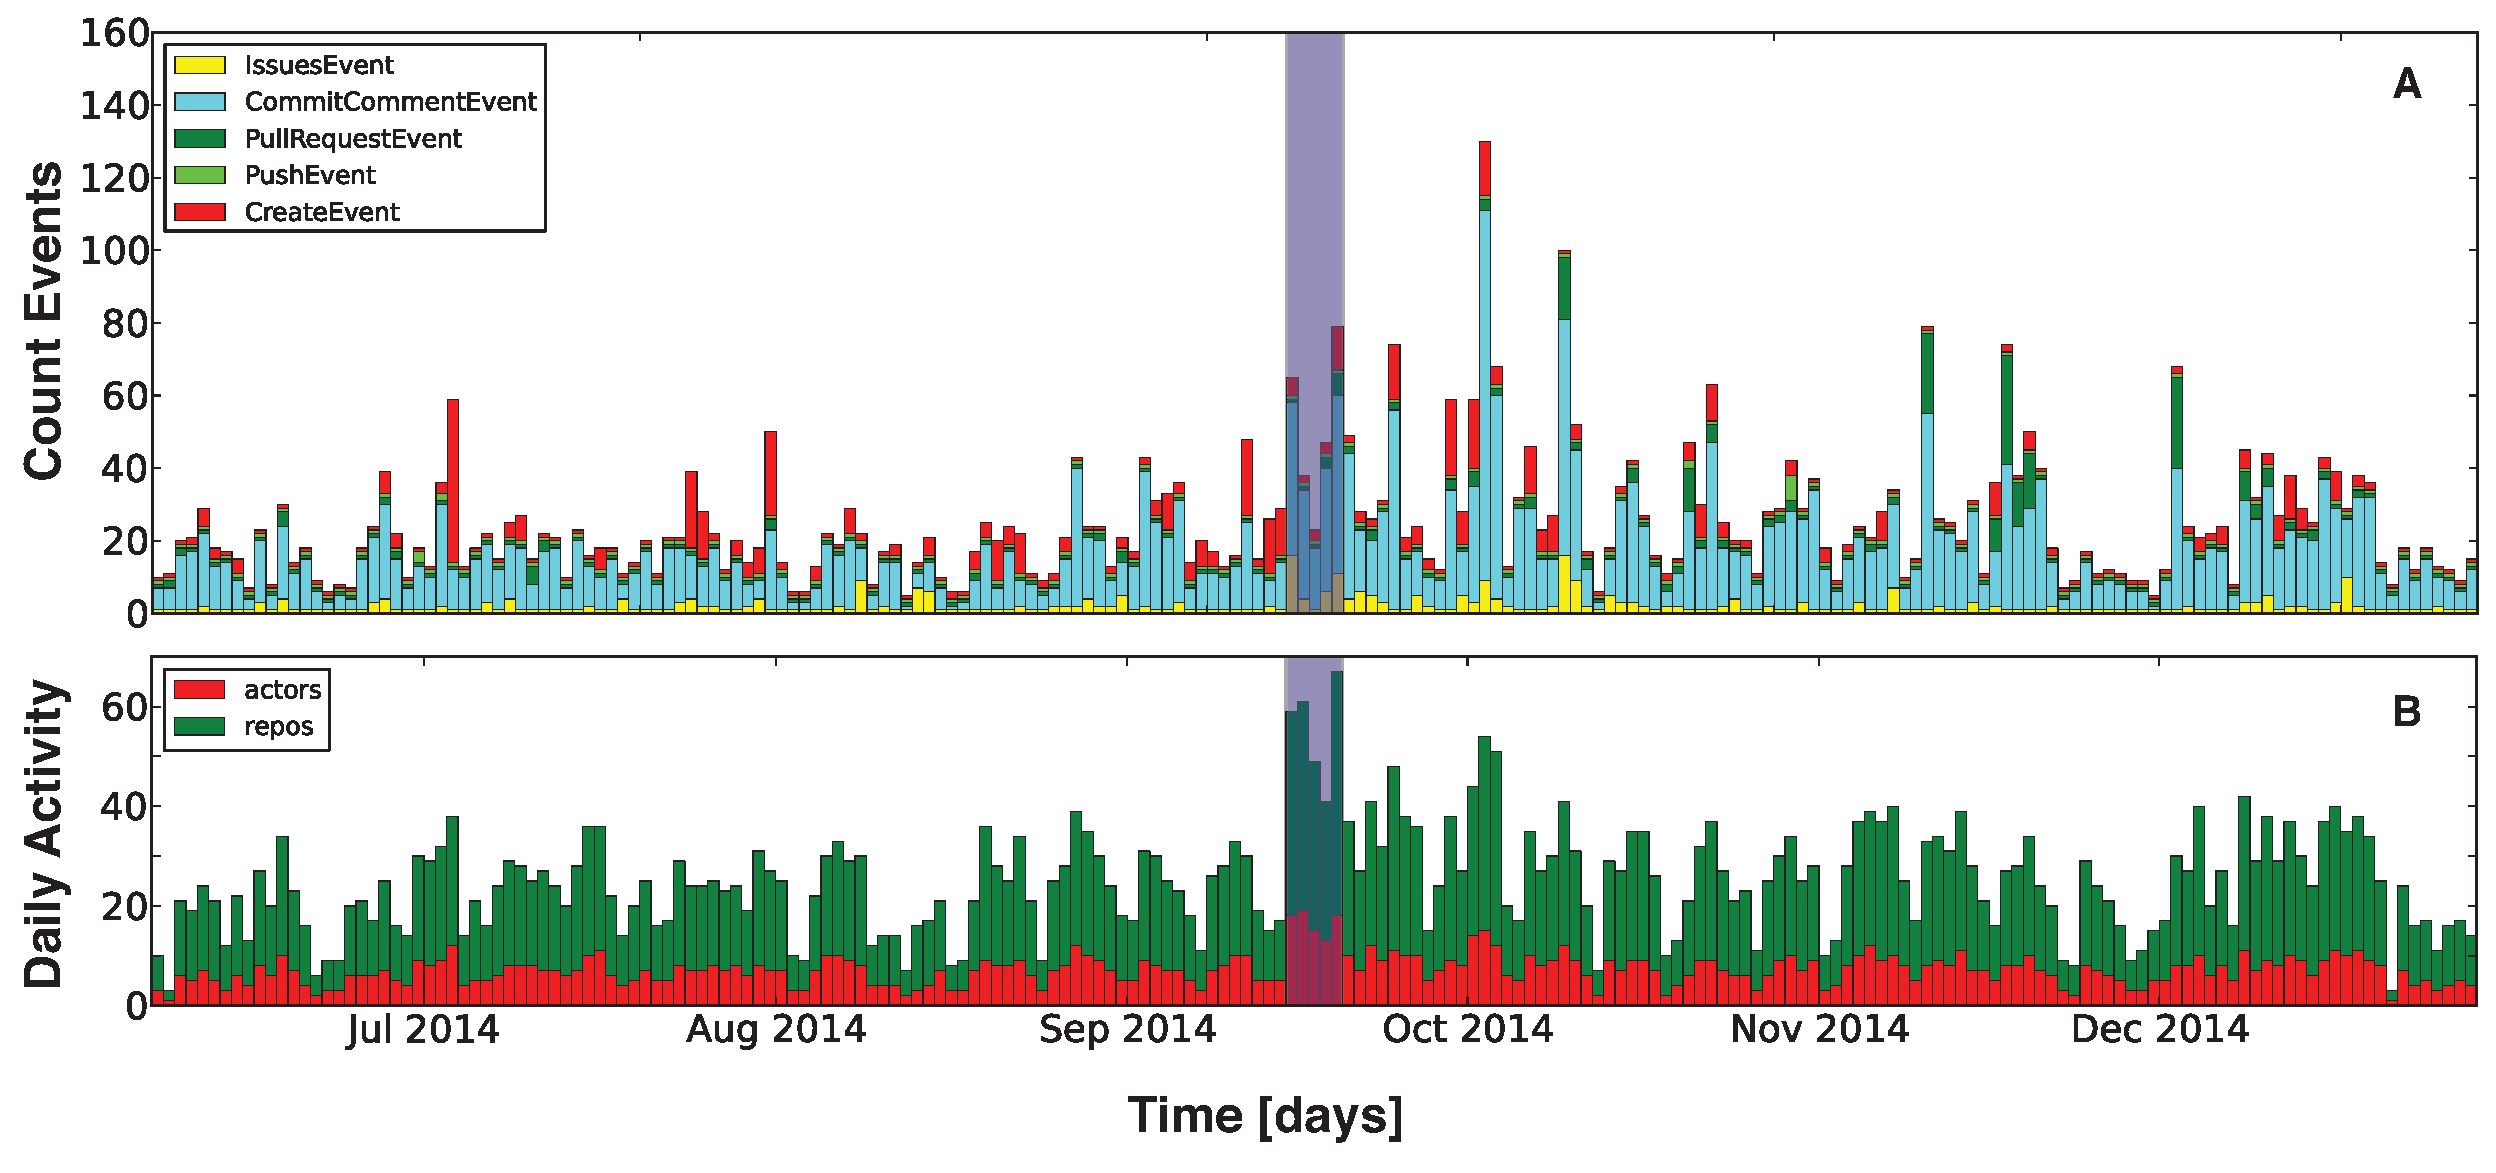
\includegraphics[width=2.0\columnwidth]{figures/timeline.eps}
\caption{ {\bf Panel A:} Histogram of daily events stacked by type, as described by the legend. The shaded purple area highlights the Astro Hack Week. {\bf Panel B:} (Stacked) daily activity of actors and repositories. The daily count of events, as well as actor and repo activity exhibit a burst during the AstroWeek, with an increase of respectively 60\%, 87\%, 53\%, compared to the average daily activity in the last 6 months before. This burst is followed by a slow decay until the end of december 2014.
%For daily active actors {\bf [repos instead?]}, the median, 75th and the 90th percentiles are reported. During the AstroWeek all days have an actor activity above the 90th percentile {\bf [Note that there is an obvious selection bias here, because we precisely study this community $\rightarrow$ it remains to be clarified why it's relevant to report this value]}, and the number of events is above the 75th percentile 4 days out of 5. While bursts of events are not rare, the coalescence of actors (and of repos), is unique over the year around AstroWeek, and shows the unique ``dynamics occurring during, and after this community building event."
}
\label{fig:time_series}
\end{figure*}

\subsection{The Astro Hack Week Impulse}
Figure \ref{fig:time_series} shows the number of events by type (panel {\bf A}), and the number of active contributors and active repositories per day (panel {\bf B}), for the 30 participants with a GitHub account. During the AstroWeek, the daily count of active participants, active repositories and events, increased by respectively $84.3\%$, $50.7\%$, and $58.4\%$. The number of new repositories created jumped from a weekly average of 7.5 (since March, 15, 2014) to 43 repositories created during the hackathon. The number of repository creations remained then sustained for nearly one month (yellow bars), showing that even after the end of the meeting, former participants have created and worked on new data science tools, beyond the initial scope. After the peak, the activity (in terms of events, active actors, or repositories) also exhibits a sustained --yet decaying-- activity until roughly 100 days after the hacking week. These slow decays are expected from empirical results in open source software communities \cite{sornette2014much}, and from the theory \cite{saichev2013hierarchy}. They are key to rationalize and measure the after-effects of the Astro Hack Week.


\subsection{Long-Memory Process and Slow Activity Decay}
To better grasp these long-term and slow decaying dynamics of activity --directly and indirectly related to the AstroWeek-- we investigated decays, first considering only repositories created during the hackathon week \cite{astro_hackpad} and from \cite{astro_github}, and then all repositories created by the community after the AstroWeek.

Figure \ref{fig:decay_astro_repos} shows the relaxation of activity directly related to the Astro Hack Week, over the 100 days following $t_0$, i.e., September 15th, 2014. In double logarithmic scale, we observe negative linear slopes, which confirm the power law relaxation after an exogenous shock, given by equation (\ref{eq:critical_decay}). The decay exponents $\alpha$ for daily count of active actors and contributed repositories are similar ($alpha = 0.60\pm0.08$), while the number of events per day decays faster, with exponent $0.87\pm0.14$, yet from a higher peak (close to 100 events at $t_0$). The average decay of number of events per actor (resp. repository) is obtained as $\sim 1/(t-t_0)^{\beta}$ with $\beta \approx (0.87 - 0.60) = 0.27$. Thus, after 100 days, the activity per actor (or per repository, since in both cases $\alpha \approx 0.60$), is still $30\%$ of the activity per actor at $t_0$. At the same time ($t=100$), the number of actors active on repositories created during the AstroWeek is only $6.30\%$ of its peak activity, and the number of events is nearly $1.8\%$ of initial activity (i.e., roughly 100 events per day). In other words, the activity directly related to the AstroWeek has become nearly residual after 100 days.

We now turn to activity un-conditioned (i.e., not directly related to the Astro Hack Week), but triggered by the community building effect. Figure \ref{fig:relaxation} shows the relaxation of activity (again in double logarithmic scale) over the 100 days following the AstroWeek. We observe negative linear slopes, which confirm again the power law relaxation given by (\ref{eq:critical_decay}) after $t_0$. For daily events, actors and repository activity, the exponents $\alpha$ are roughly the same (respectively $0.28\pm0.08$, $0.22\pm0.05$,$0.21\pm0.05$). The un-conditioned decay, in comparison with Figure \ref{fig:decay_astro_repos}, is much smaller. For the matter of illustration, taking $\alpha = 0.25$, the remaining activity after $100$ (resp. $1000$, $10^5$) days, is $31.6\%$ (resp. $17.8\%$, $10\%$) of the initial peak activity. Thus, in theory, even after an arbitrary long period, the follow-up activity triggered by the AstroWeek is likely to remain significant. For instance, after $100$ days (resp. $1,000$ days), $13$ (resp. $7$) out of $43$ average daily events, i.e., $30\%$ (resp. $16\%$), may be considered as direct and indirect follow-up events of the AstroWeek. 

The apparent long-term influence of the the Astro Hack Week is remarkable, and deserves further scrutiny, in order to identify its origins. Figure \ref{fig:relaxation} shows also the decay of the weekly count of repository creations (black circles). Yet the decay follows a much faster power law relaxation with exponent $0.60\pm0.10$ -- compared to the daily count of actors, repositories, and events -- its after-effects are not negligible, considering that each repository triggers follow-up activity. If we consider that creating a repository is an originating event, from which events are triggered, hence generating follow-up activity from one or several actors, then, we can interpret the slow-decaying dynamics of the AstroWeek as the combined effect of an exogenous critical triggering of repositories and the long-memory decay of activity of repository created. {\bf [here, I could do a quick numerical verification that these repositories, indeed trigger events]}. 

%follows: repositories are created following $\sim A_{t_0}/(t-t_0)^{\alpha}$ with $\alpha \approx 0.6$. {\bf [I think this is wrong : ``Then, each repository triggers activity on average as $\sim 1/(t-t{0})^{\gamma}$ with $\gamma \approx 0.6 - 0.28 = 0.32$." $\rightarrow$ here, there is a special renormalization of the exponent $\rightarrow$ We shall maybe not enter here in this paper]}.

%{\bf [Say something on super-linear productive bursts, and the fact that the Astro Hack Week looks like a burst, yet with a similar structure of contributions?]} 

%What has changed after these 100 days? look at activity resume after Holidays (i.e., January 15th) ?  {\bf [End of year should be considered as a sufficiently significant event]}.


\begin{figure}[!t]
\centering
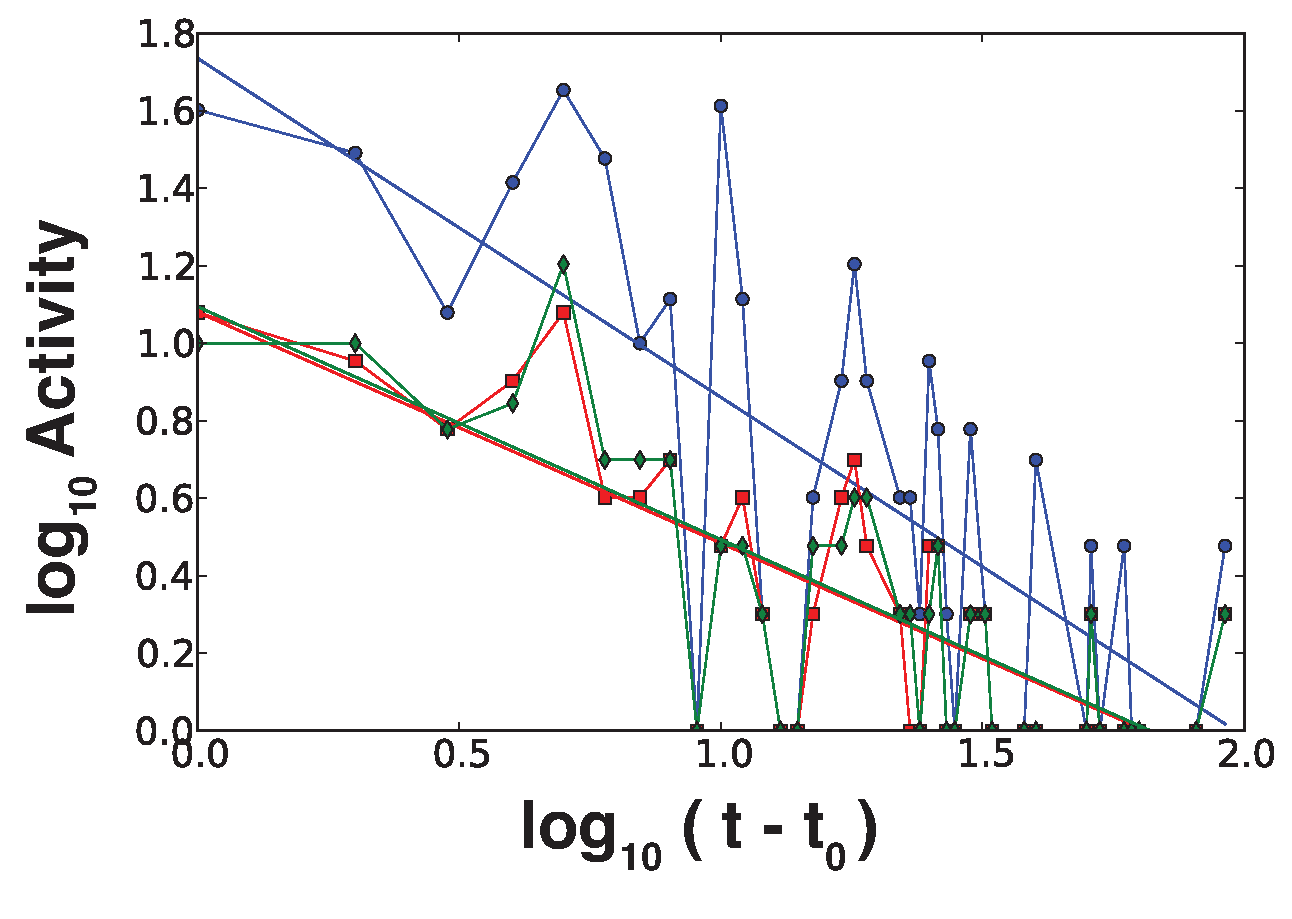
\includegraphics[width=0.9\columnwidth]{figures/relaxation_aw_repos.eps}
\caption{Decay (in double logarithmic scale) of daily activity on Astro Hack Week repositories only: actors (red), repositories (green), and events (blue). All activity types are fitted with power law decay following formula (\ref{eq:critical_decay}), with very similar exponents for actors, and repositories ($alpha = 0.6\pm0.08$). The relaxation of the daily events is much faster with exponent $0.87\pm0.14$. Comparison with Figure \ref{fig:relaxation} shows that actors, have rapidly started to work on other repositories, slightly less related to the Astro Hack Week, yet they have not abandoned the projects started during the period Sept. 15--20, 2014.}
\label{fig:decay_astro_repos}
\end{figure}

\begin{figure}[!t]
\centering
\includegraphics[width=0.9\columnwidth]{figures/relaxation.eps}
\caption{Decay (in double logarithmic scale) of daily activity after the start of the Astro Hack Week ($t_0 = $ september 15th, 2015): actors (red), repositories (green), events (blue) and weekly creation of repositories (black circles). All activity types are fitted with power law decay as formula (\ref{eq:critical_decay}), with very similar exponents $alpha$ for actors, repositories and events: respectively $0.22\pm0.05$, $0.21\pm0.05$, and $0.28\pm0.08$. The decay of created repositories is however faster with exponent $0.60\pm0.10$.}
\label{fig:relaxation}
\end{figure}


\subsection{Reorganization of the Distribution of Contributions}
From \cite{sornette2014much}, we know that the number of events $R$ per time window is a super-linear function,

\begin{equation}
R \sim c^{\beta}
\label{eq:superlinear}
\end{equation}

with $c$ the number of active contributors and $\beta$ the scaling exponent typically found $\beta \approx 4/3$ in a large number of open source software projects. This law of super-linear production stems from critical cascades of individual and collective contribution events. In the case of individual contributions, cascades, lead heavy-tailed distributions (i.e., large deviation) of individual contributions. In other words, the super-linear effect observed is largely due to a few large contributors. Figure \ref{fig:tradeoff} (panel {\bf A}) shows that super-linear productive bursts of events have also occurred on a regular basis, within the AstroWeek community, before, during and after the hackathon.

However, the AstroWeek gathered both lay and seasoned data scientists. Questioned on the trade-offs implied by spending time teaching lay participants, a senior contributor (P4) answered that the AstroWeek prevented him from contributing as much as what he would routinely do. Figure \ref{fig:tradeoff} (panel {\bf B}) shows a comparison of event counts per actor during and after the AstroWeek as a function event counts per actor before the hackathon (in double logarithmic scale). While the relation between counts before and after is almost linear (scaling exponent $= 0.82\pm0.10$ close to $1$), the comparison of event counts during the AstroWeek as a function as before exhibits a scaling with $\mu = 0.35\pm0.08$, which is strongly sub-linear. In other words, while largest contributors before AstroWeek are still the most contributing actors during the AstroWeek, the number of their contributions is marginally decreasing, confirming the statement provided by interviewee P4. Yet contributions remain bursty during AstroWeek, so events not contributed by senior actors, seem to be --at least partly-- compensated by less senior actors. This contribution gap may be further identified by considering that while the number of daily active participants increased by $84.3\%$ during the AstroWeek, the number of events increased by only $58.4\%$ (also clearly visible on Figure \ref{fig:time_series}).

\begin{figure}[!t]
\centering
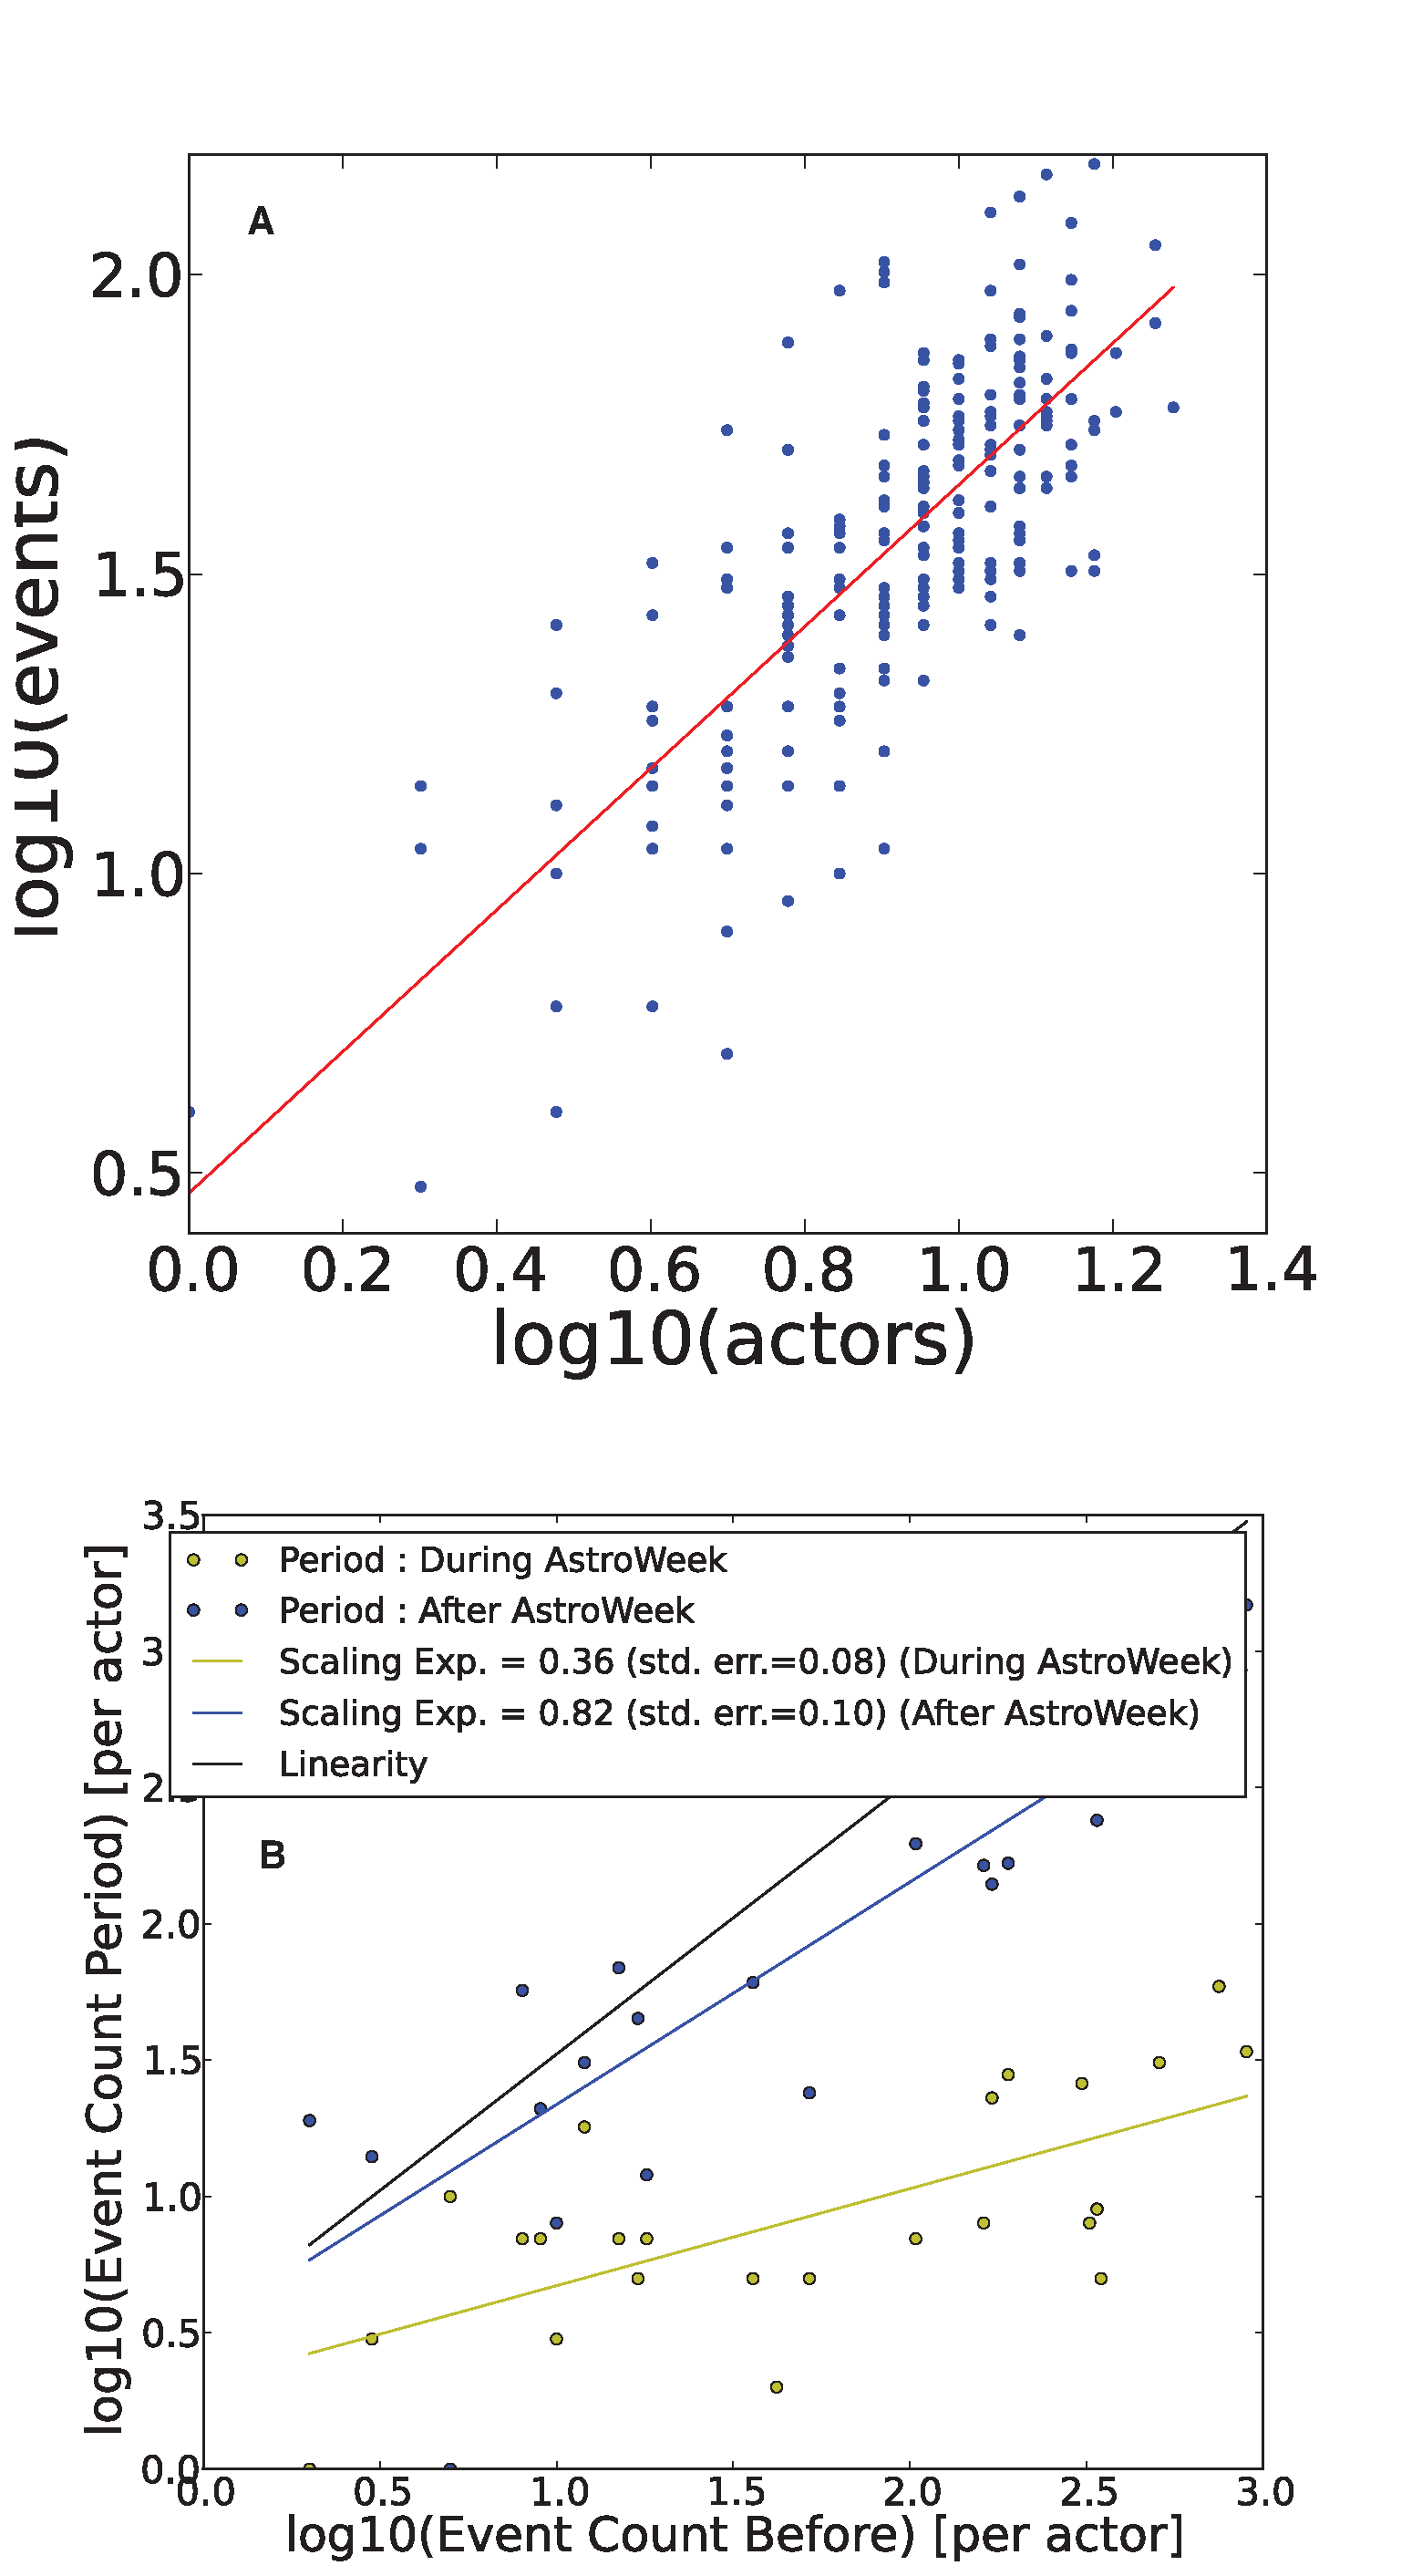
\includegraphics[width=0.9\columnwidth]{figures/tradeoff_senior_contributors.eps}
\caption{{\bf Panel A: } Count of events as a function of active actors per day (in double logarithmic scale). This relation exhibits a scaling given by equation \ref{eq:superlinear}, with exponent $\beta = 1.18 \pm 0.06$. After the Astro Hack Week the same relationship holds with exponent $1.18 \pm 0.07$ (not shown). {\bf Panel B: } Comparison of event counts per actor during and after the Astro Hack Week as a function of event count per actor before the hacking week. The amount of contributions exhibits a marginal decrease, characterized by the scaling exponent $\mu \approx 0.33 < 1$, i.e., following a sub-linear function of individual contributions during the Astro Hack Week as a function of individual contributions before. For reference, the count of contributions {\it after}  as a function of {\it before} the AstroWeek, is also presented, and appears to be very close to linearity (scaling exponent close to 1).}
\label{fig:tradeoff}
\end{figure}

Our results show that the Astro Hack Week had an {\it impulse} effect on the community, followed by mid-term and long-term spillovers, which can be measured precisely using the response function given by equation (\ref{eq:critical_decay}), with exponent $\alpha \approx 0.6$ larger (faster decay) for activity directly associated with the AstroWeek, and $\alpha \approx 0.25$ for activity indirectly related to AstroWeek projects. These results suggest that AstroWeek projects were rapidly abandoned and gave way to more heterogeneous contributions on GitHub, reflecting the increased exploration of the capabilities of open and reproducible science, by the actors having participated in the hackathon. The trade-offs faced by senior actors --when the teach instead of practicing open and reproducible science-- show that the community has undergone a punctual re-organization of the distribution of contributions during the Astro Hack Week.


%For example, taking a power law decay with exponent $\alpha = 0.25$, the remaining activity after $100$ (resp. $1000$) days, is $31.6\%$ (resp. $17.8\%$) of the initial peak activity. Note that with a larger power law exponent, such as $\alpha =0.60$ comparable to the decay of created repositories, the remaining activity is small after $100$ days  ($6.3\%$) and residual after $1000$ days ($1.5\%$). Thus, the value of the power law exponent $\alpha$ plays a critical role to measure the mid- and long-term after-effects of a punctual event, such as the Astro Hack Week.

%{\bf [add a study of events which are directly related to Astro Hack Week, versus peripheral events, (which by the way may be far more important)]}

%We distinguish three typical dynamics:
%- dynamics related to actions taken in relation with astro week (astro week actors, astro week repos)  (critical yet relatively short memory process)
%- dynamics related to actions taken by astro week actors, on indirectly related repositories (much longer memory process)  {\bf [check that the much longer memory process is not due to the addition of the latter to the former]}.
%- productive bursts, how they connect with the two former results, and how they offer a universal measure of the community, regardless of the exogenous Astro Hack Week event.


\section{Discussion}
To understand how open and reproducible data science operates ``under the hood" through critical triggering dynamics, we have measured the response activity following the impulse of the Astro Hack Week , a one week hackathon for astronomers. Our results help describe the complex dynamics, behaviors and tradeoffs faced by the actors of this community, which deserve bringing a broader context. They also open new questions for future research directions.

Our approach, which combines in-depth modeling of actions taken by participants and their dynamics, before, during and after the AstroWeek, with a typical qualitative gathering of ethnographic evidence, brings a broad context view of the long-memory dynamics observed. We have characterized a {\it kairos} moment \cite{orlikowski2002s} of open and reproducible science, focused on community joining and integration, with non trivial spillovers and long-term effects. Nevertheless, our observations suggest that the initial shock, namely, the first day of the AstroWeek, or at least the AstroWeek itself, gives the impulse. Therefore, at least in theory, the larger the initial impulse the more important the long-term response. There are two ways to enhance this peak activity: Either increase the number of participants, or find ways to increase activity with the same number of participants. In practice, tuning the impulse as a parameter, may be more tricky: More participants increase coordination costs, and it is unclear how to boost activity. The impulse may also be conditioned to previous exposure to  collaboration and social interactions.

Similarly, although the exponent $\alpha$, representing the long-memory response (the lower $\alpha$, the slower the decay) seems to be stable and robust across activity types, it remains unclear whether we observed a genuine feature of the AstroWeek, of a more general law of open and reproducible science, or a universal law of open collaboration. The origin of the small exponent ($\alpha \approx 0.25$) requires more investigation. It may stem from the combined effects of cascades of repository creations and critical triggering of contributions. It may also result from complex networks of influence between community members, and even types of events \cite{saichev2013hierarchy}. There is little doubt that the nature of events play a role in the cascading dynamics, yet it remains hard to investigate in detail. In addition, there are multitudes of {\it weak} signal, which cannot be captured either because they are systematically not recorded (e.g. talking at a pub, as shown on Figure \ref{fig:pub}), but also from the GitHub data, which might be too entangled or not significant enough to draw solid conclusions.

\begin{figure}[!t]
\centering
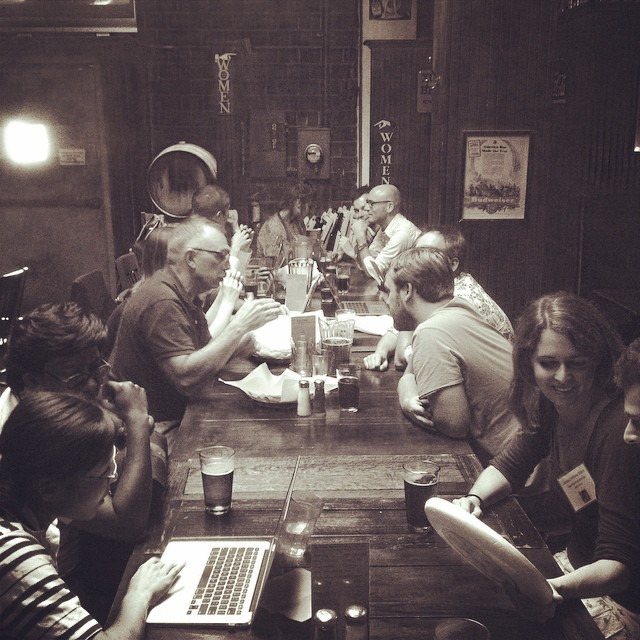
\includegraphics[width=0.9\columnwidth]{figures/pub.jpg}
\caption{Happy hours at Astro Hack Week 2014. Photo by Adrian Price-Whelan. (source: \url{http://astrohackweek.github.io/blog/astro-hack-week-wrapup.html})}
\label{fig:pub}
\end{figure}

This is precisely where the ethnography approach plays a fundamental role to provide context, not only for the dynamics observed and modeled, but also to guide the expert in quantitative social dynamics, in order to ask the good questions and search meaningful information, which might be buried in the ocean of data. For instance, an interviewed senior data scientist (P4), reported that while it was an investment for him to teach at the Astro Hack Week, this event allowed him build social ties with another senior scientist. These social ties have turned into a research project (posted as a repository on GitHub), several months later. In principle, this information could be dug out of the data, but it is less sure whether it would be worth launching a quantitative analysis on these kinds of very long-term follow-up events, without enough contextual information. Having this information in hand, new research paths on the very long-term effects of a hackathon may be quantitatively investigated in the future.

Conversely, the quantitative approach was useful for fact checking of some biased perceptions by interviewees. For instance, a participant believed that activity followed a step function, i.e. little activity before, a lot during, and again little activity after the Astro Hack Week. He was not conscious that follow-up activity really existed in the way we have described.

More broadly, each hackathon is a unique experience bringing its own kind of people. It remains to be seen how the results presented here generalize, and on the contrary, how they constitute the footprint of the Astro Hack Week. Similarly, a larger sample of investigated hackathons would help better identify the rules commons of all hackathons, and at the same time, their unique specificities.

Although GitHub, as well as other social coding platforms, has proven to be very efficient platforms for open and reproducible science collaboration, efforts have been undertaken for a better integration of tools for computational science. For instance, the IPython Notebook has been credited to be ``great for working through things interactively, virtually all [my] work starts here.� Very recently, GitHub has integrated the IPython Notebook viewer (i.e., NB viewer) in its interface, in order to visually render all notebooks stored in GitHub \cite{notebook_rendering}. This example opens the question of the importance of tools in the open and reproducible science process, and how their evolution may additionally change the practice of science. As the practice of science change on open collaboration platform, we shall also witness the evolution of activity patterns, when considering the underlying software used by scientists. Further investigation is necessary to delineate how these increasingly online and web based tools will actually impact the science practice, and whether it is possible to anticipate the evolution of these tools.


%For example, a pattern recognition tool for search and identification of stars, developed by astronomers, may be repurposed for mapping aerial satellite images \cite{kapadia} {\bf [not sure if this example is best]}.

%- find long-term traces of activity (common projects may be initiated months after initial physical meeting $\rightarrow$ kyle interview saying that he has started something with Phill Marshall). Resonates with the very slow (theoretical) decay.


%It's unclear how the social ties established on the long term, triggering collaboration between a subset of the community several months or even years after the Astro Hack Week, may be traced back through the empirical dynamics, to the original encounter. However, the structure interview may greatly help bridge this gap. For instance, when asked about long-term spillovers and benefits of the Astro Hack Week, a senior participant indicated that he started a research project in collaboration with two other senior data scientists, whom he had met and got to know during the Astro Hack Week. Such indication, may help trace meaningful ties between events, which otherwise would be buried into the ambient activity, and for which getting statistical significance of causality, may simply be impossible.


%one point statistics: we shall see it what fashion it will repeat in Astro Hack Week 2015, or in similar events. We shall not presume that all events have the same response dynamics (we have preliminary evidence that another event, involving the astro community has happened earlier in 2014, with slightly different dynamics). We shall on the contrary leverage our proposed method combining quantitive modeling with structured interviews, to bring deep insights, on the complex dynamics and social interactions, occurring during data science events.

%\section{Limitations \& Future Work}











\section{Conclusion}
With the development of open and reproducible science, new research practices have emerged. These practices rely on writing software and libraries for the purpose of solving scientific problems, often associated with massive amount of data. To help researchers familiarize with this {\it new way} of doing science, hackathons are increasingly organized. Here, we studied the dynamics triggered by the Astro Hack Week 2014. We found that past the initial impulse, involving a trade-off for senior data scientists, the community triggered mid- and long-term follow-up activity, with long-term activity being more related to the acquisition of this new science practice. 

In our respective academic traditions, social science and complexity science, information could be dug out of our different data collection processes. On the one hand, for the quantitative analysts, it is questionable whether it would be worth launching a quantitative analysis of this kind with very long-term follow-up events, without gathering enough contextual information. On the other hand, for the qualitative researcher, quantitative theories and modeling provide predictive models of activity and social interactions, which in turn can be observed in field research. In the future we hope to integrate more critical thinking: The ethnographic approach plays a fundamental role to provide context and critical analysis of the dynamics observed. At the same time, the quantitative approach helps frame qualitative questions and target meaningful ethnographic information retrieval. Our approach, combining quantitative and qualitative methods, may thus further help enrich research in Science, Technology and Society (STS), and in complex system dynamics, both focused on the emergence of collaborative approaches to the practice of science.



%With the development of open and reproducible science, new research practices have emerged. These practices rely on writing software and libraries for the purpose of solving scientific problems, often associated with massive amount of data. To help researchers familiarize with this {\it new way} of doing science, hackathons are increasingly organized. Here, we studied the dynamics triggered by the Astro Hack Week 2014. We found that past the initial impulse, involving a trade-off for senior data scientists, the community triggered mid- and long-term follow-up activity, with long-term activity being more related to the acquisition of this new science practice. Our research approach combined quantitative modeling of social dynamics, and gathering of ethnographic materials. This approach has proven cross-nurturing, and may further help enrich research in Science, Technology and Society (STS), focused on the emergence of collaborative approaches to the practice of science.


%\begin{figure}[!t]
%\centering
%\includegraphics[width=0.9\columnwidth]{Figure1}
%\caption{For images, be sure to have a good resolution image
%  (see item D within the preparation instructions).}
%\label{fig:figure1}
%\end{figure}


%\begin{table}[!b]
%  \centering
%  \begin{tabular}{|c|c|c|}
%    \hline
%    \tabhead{Objects} &
%    \multicolumn{1}{|p{0.3\columnwidth}|}{\centering\tabhead{Caption --- pre-2002}} &
%    \multicolumn{1}{|p{0.4\columnwidth}|}{\centering\tabhead{Caption --- 2003 and afterwards}} \\
%    \hline
%    Tables & Above & Below \\
%    \hline
%    Figures & Below & Below \\
%    \hline
%  \end{tabular}
%  \caption{Table captions should be placed below the table.}
%  \label{tab:table1}
%\end{table}

% Use figure* for figures spanning the whole page
%\begin{figure*}[!t]
%\centering
%\includegraphics[width=2.0\columnwidth]{Figure2}
%\caption{Sample of a wide figure. Be sure to place at the top of the page or bottom of the page.}
%\label{fig:figure2}
%\end{figure*}

%\section{Acknowledgments}
%add ack here


% Balancing columns in a ref list is a bit of a pain because you
% either use a hack like flushend or balance, or manually insert
% a column break.  http://www.tex.ac.uk/cgi-bin/texfaq2html?label=balance
% multicols doesn't work because we're already in two-column mode,
% and flushend isn't awesome, so I choose balance.  See this
% for more info: http://cs.brown.edu/system/software/latex/doc/balance.pdf
%
% Note that in a perfect world balance wants to be in the first
% column of the last page.
%
% If balance doesn't work for you, you can remove that and
% hard-code a column break into the bbl file right before you
% submit:
%
% http://stackoverflow.com/questions/2149854/how-to-manually-equalize-columns-
% in-an-ieee-paper-if-using-bibtex
%
% Or, just remove \balance and give up on balancing the last page.
%
\balance

% If you want to use smaller typesetting for the reference list,
% uncomment the following line:
% \small
\bibliographystyle{acm-sigchi}
\bibliography{bib/astrohackweek}
\end{document}
